\newpage % Rozdziały zaczynamy od nowej strony.
\section{Warstwy}

\subsection{DENSE}
%todo:
// todo: opisać
\subsection{CNN}

% https://towardsdatascience.com/text-classification-rnns-or-cnn-s-98c86a0dd361
% https://towardsdatascience.com/a-comprehensive-guide-to-convolutional-neural-networks-the-eli5-way-3bd2b1164a53

% http://www.wildml.com/2015/11/understanding-convolutional-neural-networks-for-nlp/

Sieci używające CNN z reguły wykorzystywane są w ramach analizy obrazu. Działają one w oparciu o różne filtry przemieszczające się systematycznie po macierzy obrazu. Dany obraz może być jednocześnie analizowany przez wiele filtrów przemieszczających się z różnym skokiem. Pozwala to na naukę rozpoznawania różnych cech obrazu umożliwiających zagadnienia klasyfikacji. Kolejne warstwy CNN można ze sobą łączyć pozwalając na rozpoznawanie coraz bardziej zaawansowanych cech obrazu. 

W przypadku analizy tekstu macierzą wejściową dla warstwy CNN jest macierz o wymiarze AxB, gdzie A to liczba słów w zdaniu, a B to rozmiar embeddingu. Natomiast, ze względu na strukturę danych, sama ekstrakcja cech dokonywana przez filtr może przebiegać tylko w ramach wymiaru A, gdyż dane wzdłuż wymiaru B reprezentują unikalne cechy danego słowa i nie powinny być agregowane. 

%todo: opsiać max pooling ?
//todo: opsiać max pooling ? 

\subsection{RNN}

% http://colah.github.io/posts/2015-08-Understanding-LSTMs/ 

% https://towardsdatascience.com/illustrated-guide-to-recurrent-neural-networks-79e5eb8049c9 


Neuronowa sieć rekurencyjna (RNN) powstała z myślą o przewidywaniu kolejnych elementów sekwencji. Jako wejście przyjmuje kolejne elementy sekwencji, ale w przeciwieństwie do sieci typu feedforward posiada także swój wewnętrzny  stan, w ramach którego zawarta jest informacja o poprzednich wejściach. Sieć tego typu charakteryzuje się jednak bardzo istotną wadą, mianowicie boryka się ona z problem zanikającego gradientu. Jest on spowodowany naturą propagacji wstecznej i wiąże się z coraz mniejszym wpływem początkowych elementów sekwencji na wyjście modelu. Aby temu zaradzić zostały wprowadzone nowe architektury warstw, jedną z nich jest warstwa typu LSTM. 

\subsection{LSTM}

% https://towardsdatascience.com/illustrated-guide-to-lstms-and-gru-s-a-step-by-step-explanation-44e9eb85bf21

Warstwa typu LSTM składa się nuronów zawierających w sobie wiele pośrednich operacji. Poniżej zostaną omówione najważniejsze z nich.

\begin{figure}[!h]
    \label{fig:lstm_diagram}
    \centering 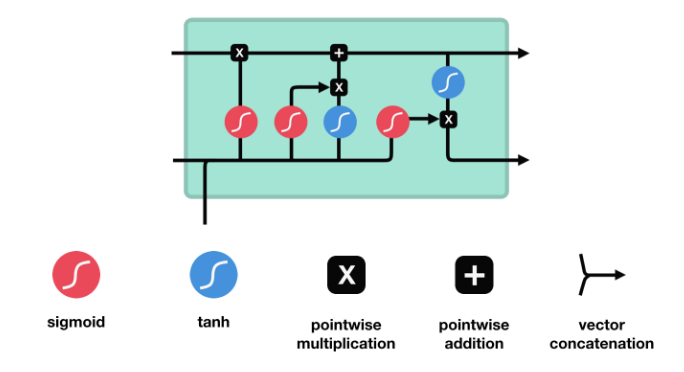
\includegraphics[width=1\linewidth]{lstm_diagram.png}
    \caption{Przepływ danych w jedynczym neuronie LSTM}
\end{figure}


\begin{figure}[!h]
    \label{fig:lstm_gates}
    \centering 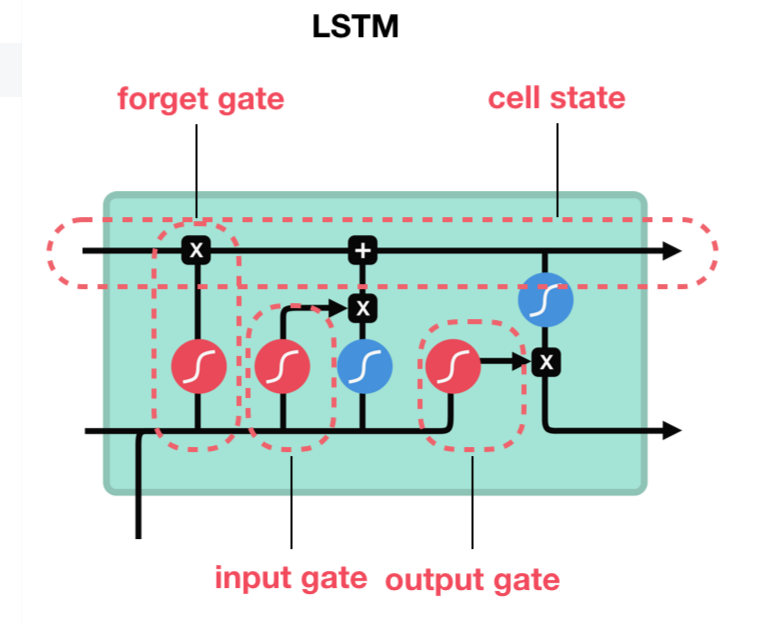
\includegraphics[width=0.5\linewidth]{lstm_gates.png}
    \caption{Przepływ danych w jedynczym neuronie LSTM}
\end{figure}


\subsubsection{Funkcje aktywacji}

Neuron LSTM wykorzystuje dwie funkcje aktywacji: 

\begin{itemize}
    \item Tahn (funkcja aktywacji typu tangens hiperboliczny) - pozwala ona na normalizowanie wektora tak by wartości zawierały się w ramach przedziału [-1,1] 
    \item Sigmoid (funkcja aktywacji sigmoidalna) - przekształca wartości wektora do wartości z przedziału [0,1]. Istotna z punktu widzenia określania, które elementy wektora powinny zostać zapamiętane (wartość bliżej 1), a które zapomniane (wartość bliżej 0) 
\end{itemize}


\subsubsection{Elementy neuronu}

W skład neuronu LSTM wchodzą następujące elementy: 
\begin{itemize}
    \item Forget gate
    \item Input gate 
    \item Cell state 
    \item Output gate
\end{itemize}
 

\paragraph{Forget gate}  \hfill
%  \break

Zadaniem tej bramy jest decydowanie jaka informacja powinna zostać zachowana przez neuron, a jaka usunięta. Informacje z poprzedniego stanu ukrytego ($h_{t-1}$) i informacje z bieżącego wejścia($x_t$) są przekazywane do sigmoidalnej funkcji aktywacji. Powstała macierz jest oznaczona jako $f_t$. Dla każdej pozycji w macierzy zwracane są wartości z zakresu [0,1]. Im bliżej wartości zero, tym wpływ danej pozycji zanika, im bliżej wartości jeden tym wpływ danej pozycji rośnie. 

 
\paragraph{Input gate}  \hfill

Służy do aktualizacji wewnętrznego stanu neuronu (‘cell state’). Informacje z poprzedniego stanu ukrytego ($h_{t-1}$) i informacje z bieżącego wejścia($x_t$) są przekazywane do sigmoidalnej funkcji aktywacji. Tak jak w przypadku 'forget gate’ uzyskiwana jest macierz o wartościach z zakresu [0,1], która tym razem określa jak bardzo informacja, powstała z połącznia $h_{t-1}$ oraz $x_t$, jest ważna z punktu widzenia zadania klasyfikacji. Wyjście z tej operacji oznaczone jest jako $i_t$. 

 W ramach tej bramy dokonuje się normalizacja informacji zawartych w ramach połączenia $h_{t-1}$ oraz $x_t$, poprzez wykorzystanie tangensa hiperbolicznego. Wyjście z tej operacji oznaczone jest jako $c_t$. 

Kolejnym krokiem jest agregacja informacji z $i_t$ oraz $c_t$ poprzez wykonanie operacji mnożenia macierzy. 

\paragraph{Cell state}  \hfill

Ten element neuronu odpowiada za jego stan wewnętrzny i jest przekazywany między kolejnymi komórkami w warstwie. Stan uzyskany z poprzedniej komórki oznaczony jest jako $c_{t-1}$, a z bieżącej jako $c_t$. W celu uzyskania bieżącego stanu komórki wykorzystywane są informacje zgromadzone w ramach poprzednich bram. W pierwszej kolejności dokonywane jest mnożenie macierzowe $c_{t-1}$ oraz $f_t$, które pozwala na usunięcie elementów macierzy nieistotnych z punktu widzenia sieci. Następnie dokonywana jest operacja dodawania uzyskanej macierzy z macierzą uzyskaną w ramach ‘input gate’. Powoduje to dodanie do stanu neuronu nowych informacji istotnych dla sieci. Stan po tej operacji jest określany zmienną $c_t$. 

 
\paragraph{Output gate}  \hfill

Zadaniem tej bramy jest określenie jak powinien wyglądać stan ukryty przekazywany do kolejnego neuronu. Stan ten zawiera informacje na temat poprzednich wejść istotnych z dla zagadnienia klasyfikacji. W ramach tej bramy dokonywane są trzy operacje. Pierwszą z nich jest podanie zagregowanych informacji z poprzedniego stanu ukrytego ($h_{t-1}$) i informacje z bieżącego wejścia($x_t$) na sigmoidalną funkcję aktywacji. W ramach drugiej operacji wewnętrzy stan neuronu (‘cell state’) jest normalizowany przy wykorzystaniu tangesna hiperbolicznego. Trzecią operacją jest mnożenie macierzowe wyników dwóch poprzednich operacji, w efekcie uzyskiwany jest stan ukryty neuronu, oznaczony jako $h_t$, przekazywany do następnego neuronu.

\subsection{Bi-LSTM}

%https://medium.com/@raghavaggarwal0089/bi-lstm-bc3d68da8bd0 

Warstwa składa się z dwóch tak samo zbudowanych warstw LSTM. Jedna z warstw przetwarza ciąg danych wejściowych od początku do końca, a druga od końca do początku. Pozwala to na naukę zależności między elementami w dwóch kierunkach, co przekłada się na większą liczbę informacji na temat sekwencji, co pozwala na szybsze i dokładniejsze trenowanie modelu.  

 



 